\documentclass[10pt]{beamer}
\usepackage{mathtools}
\usepackage{graphicx}
\usetheme{Marburg}
\usetheme{Madrid}
\usecolortheme{dolphin}


\mode<presentation>
\title{POLSAR Image Classification via Clustering-WAE Classification Model}
\author{Wen Xie \and Ziwei Xie \and Feng Zhao \and Bo Ren}

\begin{document}

\frame{\titlepage}

\begin{frame}
\frametitle{Introduction}
POLSAR - Plarimetric Synthetic Aperture Radar \\
\begin{itemize}
\item multi-channel and multi-parameter imaging radar system
\item based on AE and embeded with k-means clustering.
\end{itemize}

WAE - Wishart Auto Encoder

\begin{itemize}
\item used for redudcing error between input and output via wishart distance
\item based on auto encoder model and embeded with k-means clustering
\end{itemize}

\end{frame}

\begin{frame}
\frametitle{WAE Classification Model}
\begin{columns}
\begin{column}{0.5\textwidth}

Wishart Distance:

\begin{equation}
\min \limits _{W,b} \frac {1}{2N}\sum \limits _{i = 1}^{N} {{d_{Wishart}}\left ({ {H\left ({ {y_{i}} }\right ),H\left ({ {x_{i}} }\right )} }\right )}
\end{equation}
where,
\begin{equation} 
\begin{split}
{d_{Wishart}}\left ({ {H\left ({ {y_{i}} }\right ),H\left ({ {x_{i}} }\right )} }\right ) \\ = \\Tr\left ({ {H{{\left ({ {x_{i}} }\right )}^{( - 1)}}H\left ({ {y_{i}} }\right )} }\right ) \!+\! \ln \left |{ {H\left ({ {x_{i}} }\right )} }\right | \notag
\end{split}
\end{equation}
\end{column}

\begin{column}{0.5\textwidth}
\begin{figure}
\centering
\fbox{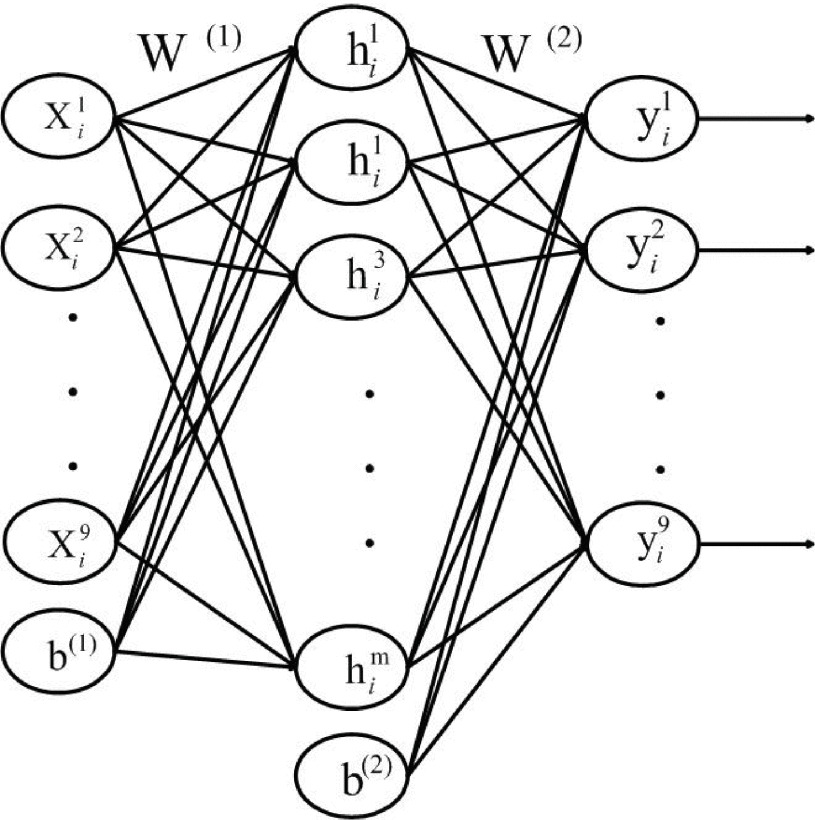
\includegraphics[scale=0.1]{figure_1.jpg}}
\caption{The structure of WAE network.}
\label{fig:one}
\end{figure}
\end{column}
\end{columns}
\end{frame}

\begin{frame}
\frametitle{Brief Review on AE Based Data Clustering}
\begin{columns}
\begin{column}{0.6\textwidth}

AE Network and K-means Clstering:

\begin{equation} 
\begin{split}
\min \limits_{W,b}~\frac {1}{N}\sum \limits _{i = 1}^{N}{{{\left \|{ {x_{i} - {y_{i}}} }\right \|}^{2}}} \\ + \lambda \sum \limits _{i = 1}^{N} {\left \|{ {f^{t}\left ({ {x_{i}} }\right ) - c_{i}^{*}} }\right \|_{F}^{2}} \\
\quad 
\hphantom {\min \limits _{W,b}~}c_{i}^{*} = \arg \min \limits _{c_{j}^{t - 1}} \left \|{ {f^{t}\left ({ {x_{i}} }\right ) - c_{j}^{t - 1}} }\right \|_{F}^{2}
\end{split}
\end{equation}

Otimization:

\begin{equation} \label{eq:three}
c_{j}^{t} = \frac {{\sum \nolimits _{x_{i} \in C_{j}^{t - 1}} {f^{t}\left ({ {x_{i}} }\right )} }}{{\left |{ {C_{j}^{t - 1}} }\right |}}
\end{equation} 
\end{column}
\begin{column}{0.5\textwidth}

\begin{figure}
\centering
\fbox{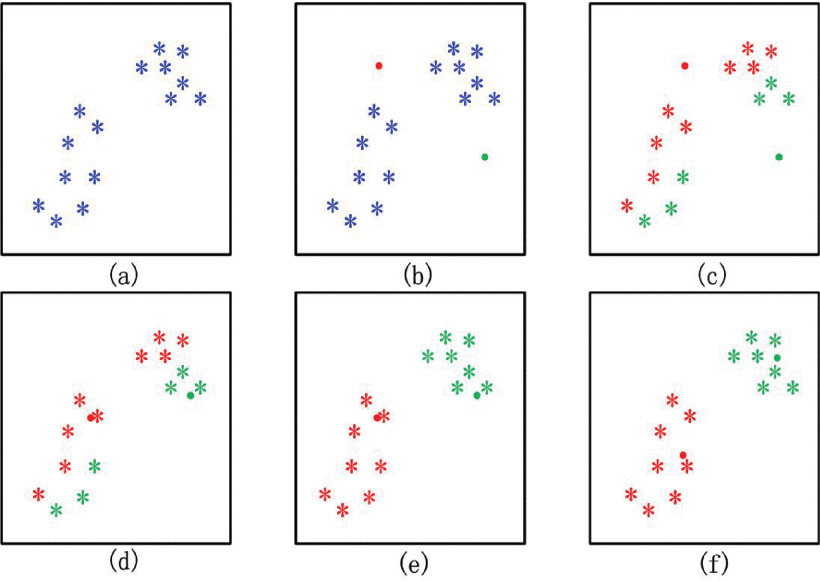
\includegraphics[scale=0.1]{figure_2.jpg}}
\caption{The schematic of K-means algorithm.}
\label{fig:two}
\end{figure}

\begin{figure}
\centering
\fbox{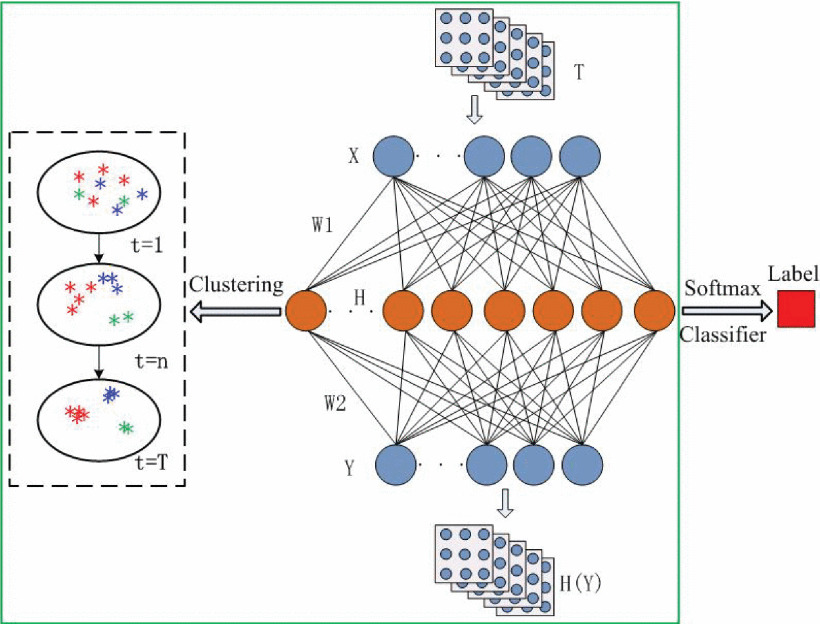
\includegraphics[scale=0.1]{figure_3.jpg}}
\caption{Framework of the our proposed method.}
\label{fig:three}
\end{figure}
\end{column}
\end{columns}
\end{frame}

\begin{frame}
\frametitle{CLUSTERING-WAE CLASSIFICATION MODEL}

\begin{equation} \label{eq:four}
\begin{split}
\langle T_i\rangle =\left[{ {\begin{array}{*{20}{c}} {T_{i}^{11}}& {T_{i}^{12}}& {T_{i}^{13}}\\ {T_{i}^{21}}& {T_{i}^{22}}& {T_{i}^{23}}\\ {T_{i}^{31}}& {T_{i}^{32}}& {T_{i}^{33}} \end{array}} }\right] \\
\to&{x_{i}} = \left [{ {x_{i}^{1},x_{i}^{2},x_{i}^{3},x_{i}^{4},x_{i}^{5},x_{i}^{6},x_{i}^{7},x_{i}^{8},x_{i}^{9}} }\right ]
\end{split}
\end{equation}

\begin{equation} \label{eq:five}
\begin{split}
\min \limits _{W,b}~\frac {1}{2N}\sum \limits _{i = 1}^{N} {{d_{Wishart}}\left ({ {H\left ({ {y_{i}} }\right ),H\left ({ {x_{i}} }\right )} }\right )} \! \!+\! \!\lambda \sum \limits _{i = 1}^{N} {\left \|{ {h_{i}^{t} - c_{i}^{*}} }\right \|_{F}^{2}} \\
\hphantom {\min \limits _{W,b}~}c_{i}^{*} = \arg \min \limits _{c_{j}^{t - 1}} \left \|{ {h_{i}^{t} - c_{j}^{t - 1}} }\right \|_{F}^{2}
\end{split}
\end{equation}

\end{frame}

\begin{frame}
\begin{columns}
\begin{column}{0.5\textwidth}
\begin{equation} \label{eq:six}
\hphantom {\min \limits _{W,b}~}c_{j}^{t} = \frac {{\sum \nolimits _{x_{i} \in C_{j}^{t - 1}} {h_{i}^{t}} }}{{\left |{ {C_{j}^{t - 1}} }\right |}}
\end{equation}

Softmax Equation:

\begin{equation} \label{eq:seven}
P\left ({ {l = j|{h_{i}};\theta } }\right ) = \frac {{{\exp ^{h_{i}^{T}{\theta _{j}}}}}}{{\sum \nolimits _{k = 1}^{K} {{\exp ^{h_{i}^{T}{\theta _{k}}}}} }}
\end{equation}
\end{column}
\begin{column}{0.5\textwidth}
\begin{table}
  \caption{Detailed Steps of Algorithm}
  \label{tab:one}
  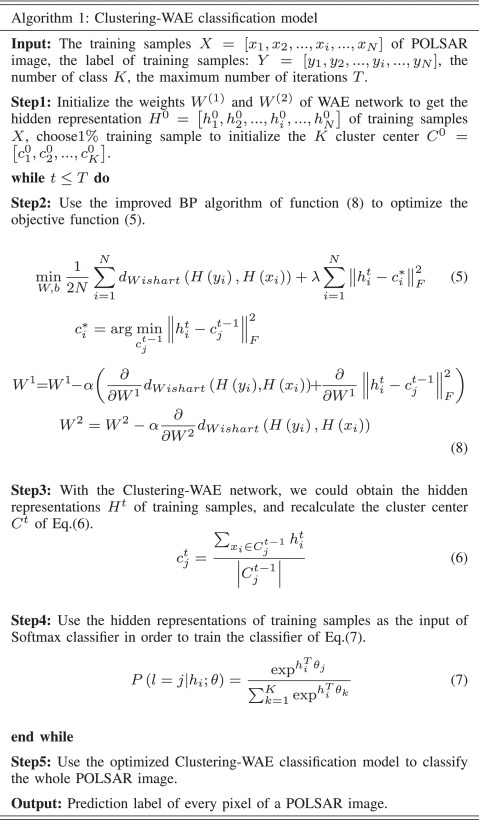
\includegraphics[width=\linewidth]{table_1.jpg}
\end{table}
\end{column}
\end{columns}
\end{frame}

\begin{frame}
\begin{columns}
\begin{column}{0.5\textwidth}
\begin{figure}
\centering
\fbox{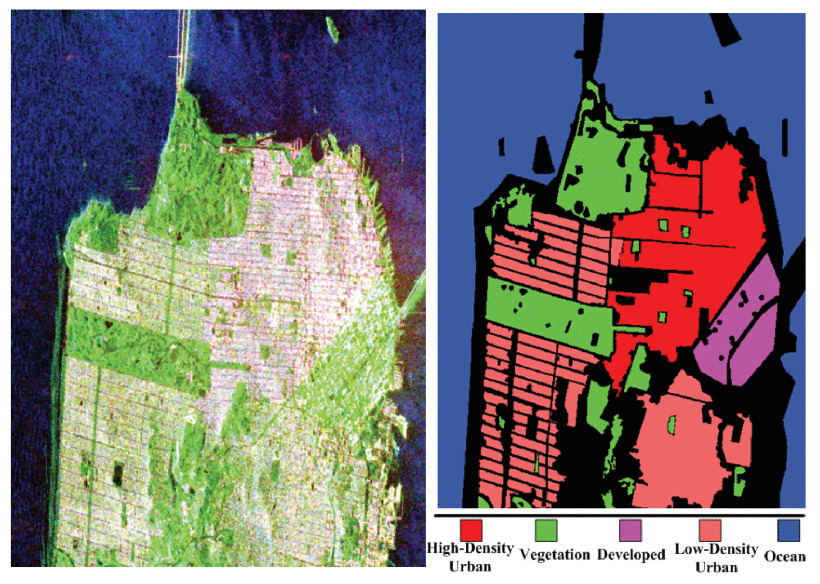
\includegraphics[scale=0.1]{figure_10.jpg}}
\caption{ Pauli RGB and ground-truth image of San Francisco.}
\label{fig:two}
\end{figure}
\end{column}
\begin{column}{0.5\textwidth}
\begin{figure}
\centering
\fbox{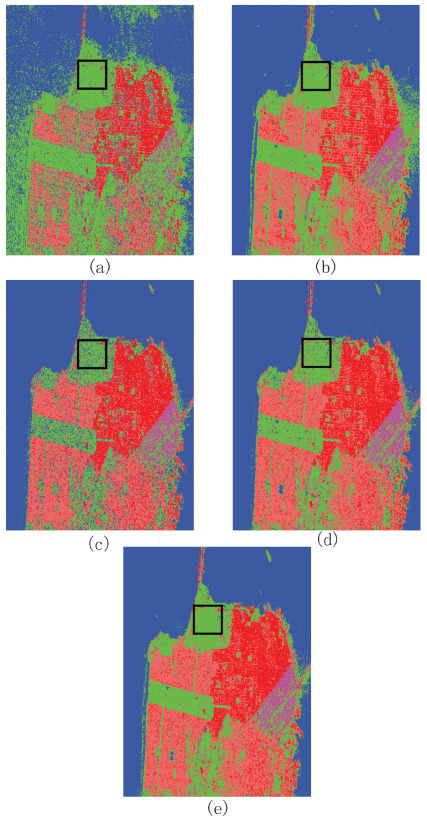
\includegraphics[scale=0.1]{figure_11.jpg}}
\caption{Classification results of different methods: K-means, Wishart, AE, WAE, and Clustering-WAE.}
\label{fig:two}
\end{figure}
\end{column}
\end{columns}
\end{frame}

\begin{frame}
\begin{table}
  \caption{Classification performances of San Francisco with different methods.}
  \label{tab:one}
  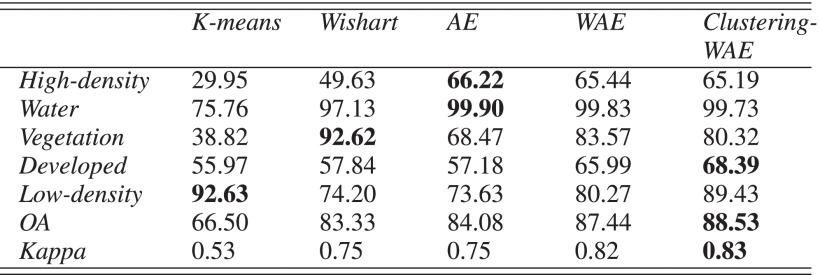
\includegraphics[width=\linewidth]{table_5.jpg}
\end{table}
\end{frame}

\end{document}